\documentclass[12pt, letterpaper]{article}
\renewcommand{\familydefault}{\sfdefault}
\usepackage[margin=1in, bottom=1.3in]{geometry}
\usepackage{amsmath,amsthm,amssymb,amscd,amsfonts}
\usepackage{mathtools}
\usepackage{enumerate}
\usepackage{multirow}
\usepackage{fancyhdr}
\usepackage{placeins}
\usepackage{graphicx}
\graphicspath{{../figures/}}
\usepackage{subcaption}
\usepackage{hyperref}
\hypersetup{colorlinks, urlcolor=blue, linkcolor=blue}
\usepackage{pdflscape}
\usepackage{bbm}

% new commands for headings and subheadings
\newcommand{\prob}[1]{\section*{Problem #1}}
\newcommand{\subprob}[1]{\subsection*{Part (#1)}}

% Edit these as appropriate
\pagestyle{fancy}
\headheight 50pt
\renewcommand{\headrulewidth}{0.4pt}
\renewcommand{\footrulewidth}{0.4pt}

\fancypagestyle{noheader}{
    \fancyhf{}% Clear header/footer
    \renewcommand{\headrulewidth}{0pt}% No header rule
    \renewcommand{\footrulewidth}{0pt}
}

\lhead{AE 598 \\ Name: Rahil Makadia \\ netID: makadia2}
\chead{\textbf{\Large Homework 1}}
\rhead{
\includegraphics[scale=0.07]{uiuc.jpeg} \\ \today}
\lfoot{}
\cfoot{\thepage}
\rfoot{}

\begin{document}
\section*{Gridworld}
The following hyperparameters were used for all algorithms unless otherwise specified:
\begin{itemize}
    \item $\gamma = 0.95$
    \item $\theta = 10^{-16}$
    \item $\alpha = 0.1$
    \item $\epsilon = 0.1$
\end{itemize}

\subsection*{Policy Iteration}
\begin{figure}[ht]
\centering
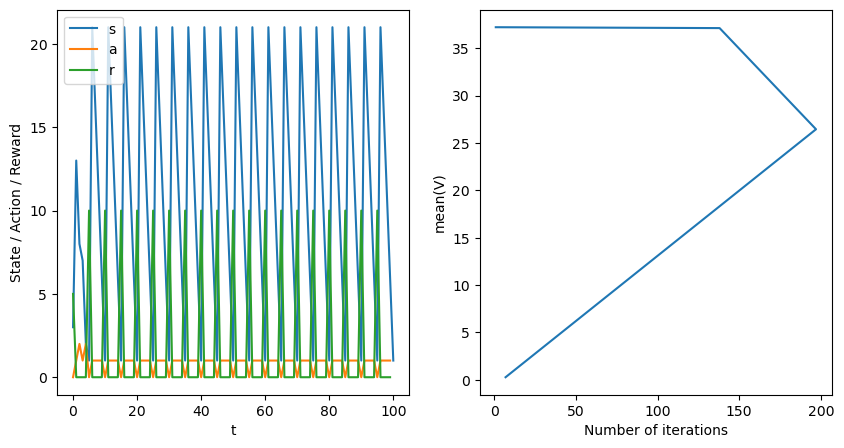
\includegraphics[width=0.8\linewidth]{gridworld/traj_return_policy_iteration.png}
\caption{Gridworld Trajectory and Learning Curve for Policy Iteration}
\label{fig:gridworld_traj_return_policy_iteration}
\end{figure}

\begin{figure}[ht]
\centering
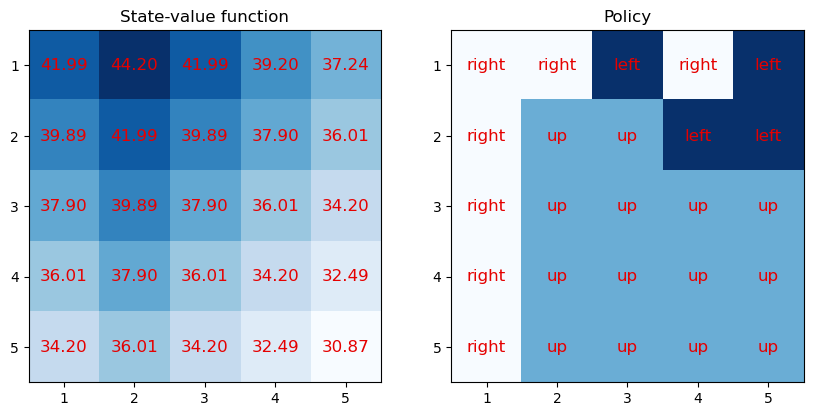
\includegraphics[width=0.8\linewidth]{gridworld/V_pi_policy_iteration.png}
\caption{Gridworld State Value Function and Policy for Policy Iteration}
\label{fig:gridworld_V_pi_policy_iteration}
\end{figure}

For the gridworld policy iteration, an example trajectory and learning curve are shown in Figure \ref{fig:gridworld_traj_return_policy_iteration}. The state value function and policy are shown in Figure \ref{fig:gridworld_V_pi_policy_iteration}. The policy iteration algorithm converges to the optimal policy in approximately 350 iterations.

\subsection*{Value Iteration}
\begin{figure}[ht]
\centering
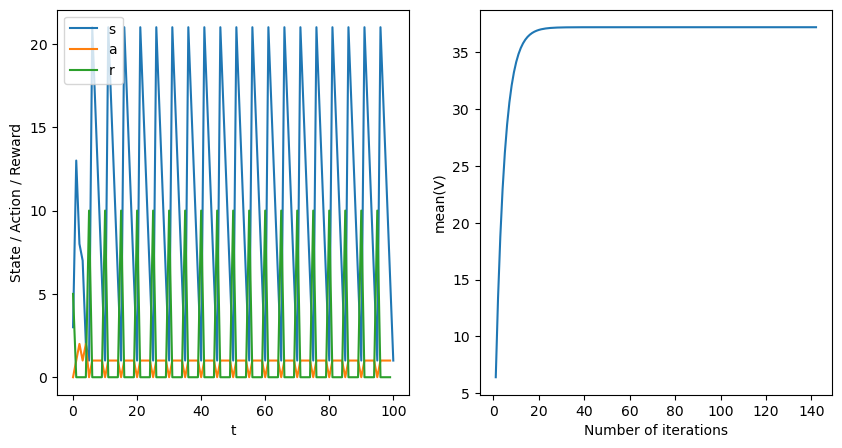
\includegraphics[width=0.8\linewidth]{gridworld/traj_return_value_iteration.png}
\caption{Gridworld Trajectory and Learning Curve for Value Iteration}
\label{fig:gridworld_traj_return_value_iteration}
\end{figure}

\begin{figure}[ht]
\centering
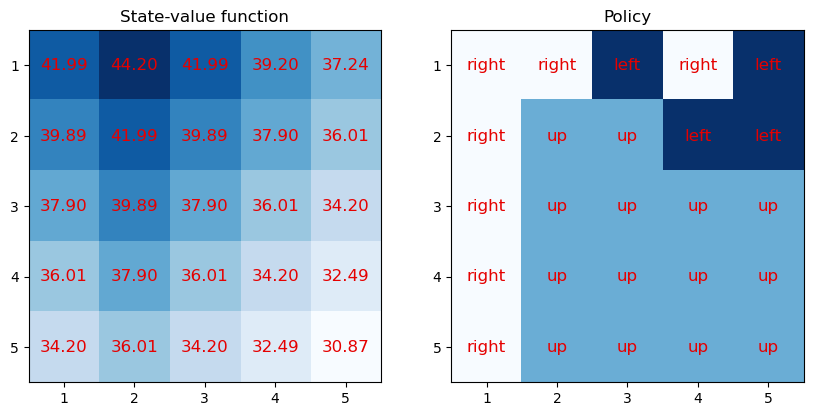
\includegraphics[width=0.8\linewidth]{gridworld/V_pi_value_iteration.png}
\caption{Gridworld State Value Function and Policy for Value Iteration}
\label{fig:gridworld_V_pi_value_iteration}
\end{figure}

For the gridworld value iteration, an example trajectory and learning curve are shown in Figure \ref{fig:gridworld_traj_return_value_iteration}. The state value function and policy are shown in Figure \ref{fig:gridworld_V_pi_value_iteration}. The value iteration algorithm converges to the optimal policy in approximately 140 iterations.

\subsection*{SARSA}
\begin{figure}[ht]
\centering
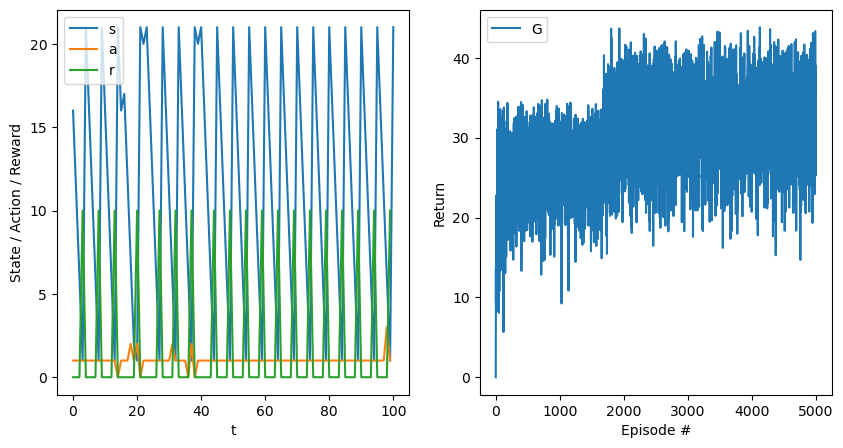
\includegraphics[width=0.8\linewidth]{gridworld/traj_return_sarsa.png}
\caption{Gridworld Trajectory and Learning Curve for SARSA}
\label{fig:gridworld_traj_return_sarsa}
\end{figure}

\begin{figure}[ht]
\centering
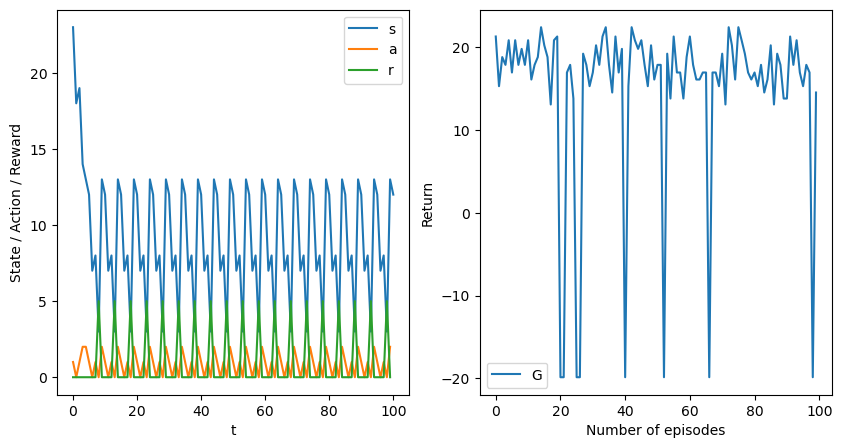
\includegraphics[width=0.8\linewidth]{gridworld/traj_return_td0_sarsa.png}
\caption{Gridworld Trajectory and Learning Curve for SARSA after TD(0)}
\label{fig:gridworld_traj_return_td0_sarsa}
\end{figure}

\begin{figure}[ht]
\centering
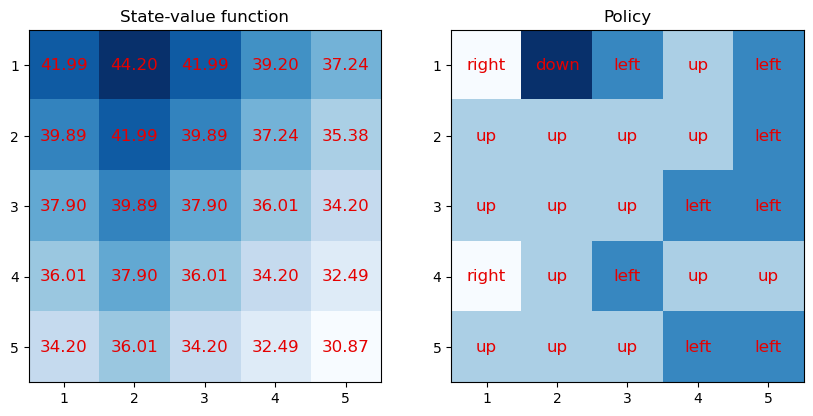
\includegraphics[width=0.8\linewidth]{gridworld/V_pi_sarsa.png}
\caption{Gridworld State Value Function and Policy for SARSA using TD(0)}
\label{fig:gridworld_V_pi_sarsa}
\end{figure}

\begin{figure}
\centering
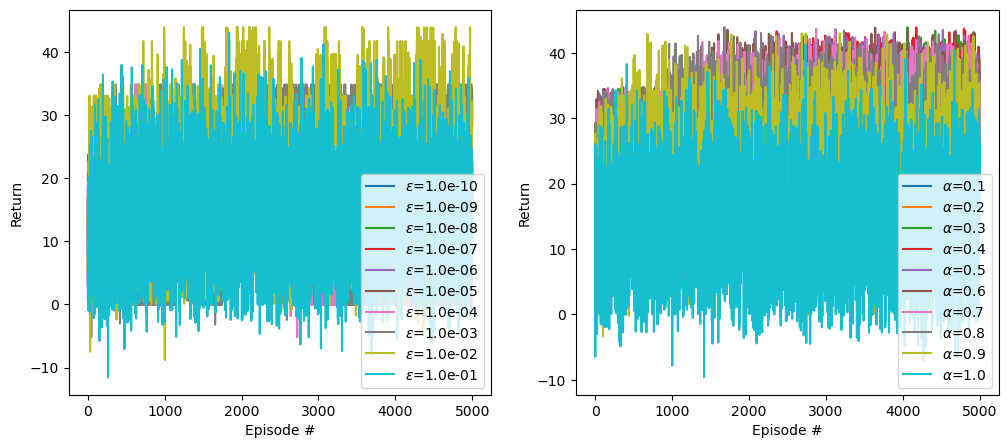
\includegraphics[width=0.8\linewidth]{gridworld/diff_epsilon_alpha_sarsa.png}
\caption{Gridworld Effect of $\epsilon$ and $\alpha$ on Learning Curve for SARSA}
\label{fig:gridworld_diff_epsilon_alpha_sarsa}
\end{figure}

For the gridworld SARSA algorithm, an example trajectory and learning curve are shown in Figure \ref{fig:gridworld_traj_return_sarsa}. The state value function and policy are shown in Figure \ref{fig:gridworld_V_pi_sarsa}. The SARSA algorithm shown here was run for 5000 episodes. Additionally, TD(0) was applied to the SARSA algorithm to derive a state value function. An example trajectory and learning curve are shown in Figure \ref{fig:gridworld_traj_return_td0_sarsa}. The state value function is nearly identical to the one generated by the value iteration and policy iteration algorithms. Additionally, the effect of varying $\epsilon$ and $\alpha$ on the learning curve is shown in Figure \ref{fig:gridworld_diff_epsilon_alpha_sarsa}.

\subsection*{Q-Learning}
\begin{figure}[ht]
\centering
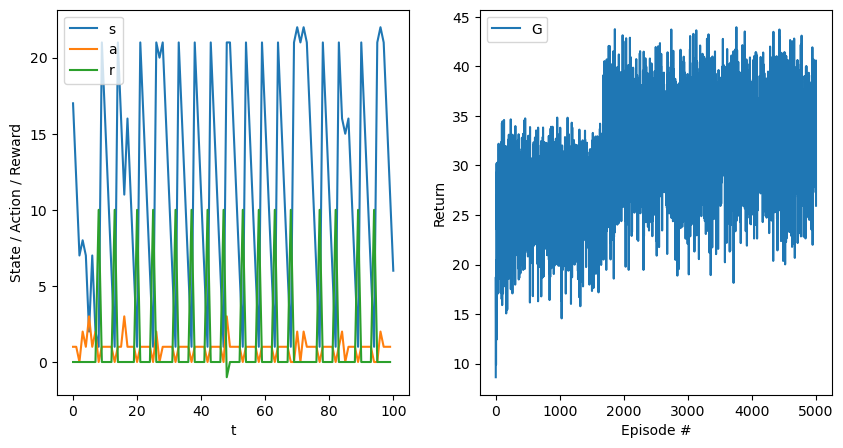
\includegraphics[width=0.8\linewidth]{gridworld/traj_return_q_learning.png}
\caption{Gridworld Trajectory and Learning Curve for Q-Learning}
\label{fig:gridworld_traj_return_q_learning}
\end{figure}

\begin{figure}[ht]
\centering
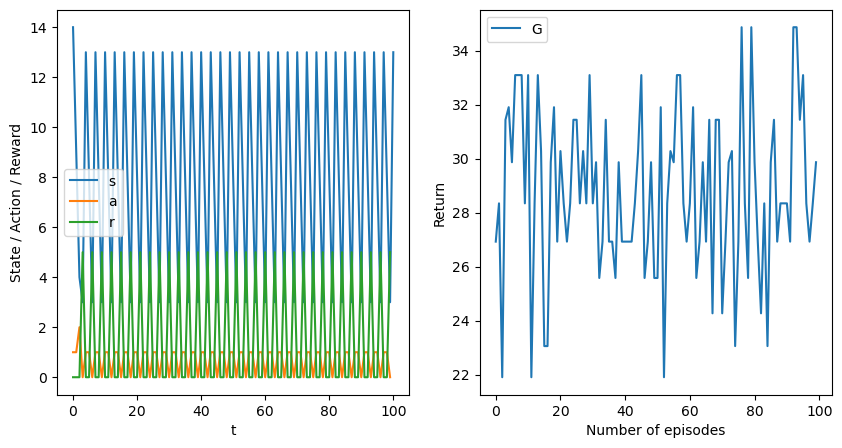
\includegraphics[width=0.8\linewidth]{gridworld/traj_return_td0_q_learning.png}
\caption{Gridworld Trajectory and Learning Curve for Q-Learning after TD(0)}
\label{fig:gridworld_traj_return_td0_q_learning}
\end{figure}

\begin{figure}[ht]
\centering
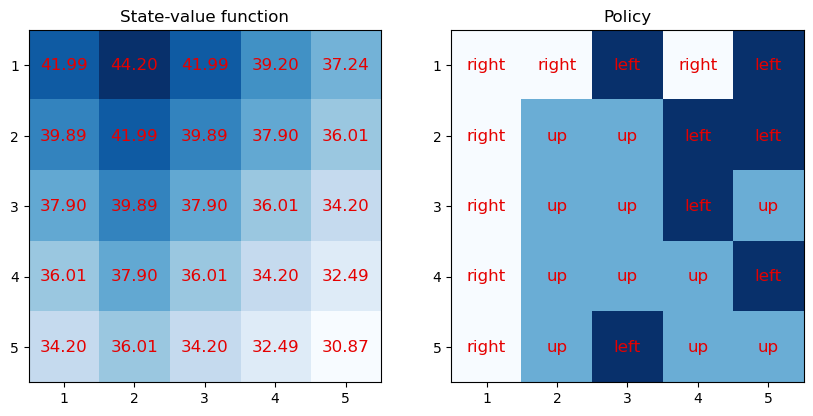
\includegraphics[width=0.8\linewidth]{gridworld/V_pi_q_learning.png}
\caption{Gridworld State Value Function and Policy for Q-Learning using TD(0)}
\label{fig:gridworld_V_pi_q_learning}
\end{figure}

\begin{figure}
\centering
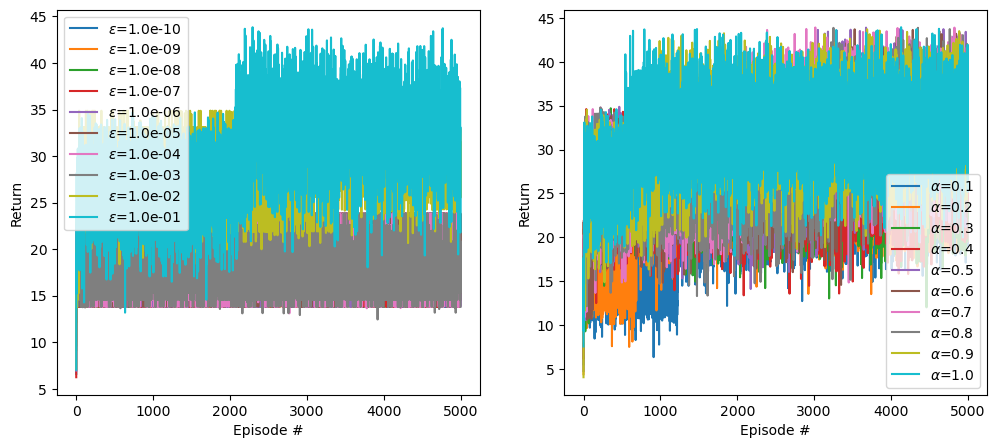
\includegraphics[width=0.8\linewidth]{gridworld/diff_epsilon_alpha_q_learning.png}
\caption{Gridworld Effect of $\epsilon$ and $\alpha$ on Learning Curve for Q-Learning}
\label{fig:gridworld_diff_epsilon_alpha_q_learning}
\end{figure}

For the gridworld Q-learning algorithm, an example trajectory and learning curve are shown in Figure \ref{fig:gridworld_traj_return_q_learning}. The state value function and policy are shown in Figure \ref{fig:gridworld_V_pi_q_learning}. The Q-learning algorithm shown here was run for 5000 episodes. Additionally, TD(0) was applied to the Q-learning algorithm to derive a state value function. An example trajectory and learning curve are shown in Figure \ref{fig:gridworld_traj_return_td0_q_learning}. The state value function is nearly identical to the one generated by the value iteration and policy iteration algorithms. Additionally, the effect of varying $\epsilon$ and $\alpha$ on the learning curve is shown in Figure \ref{fig:gridworld_diff_epsilon_alpha_q_learning}.

\FloatBarrier

\section*{Pendulum}
The following hyperparameters were used for all algorithms unless otherwise specified:
\begin{itemize}
    \item $\gamma = 0.95$
    \item $\alpha = 0.3$
    \item $\epsilon = 0.8$
    \item n$_{\theta}$ = n$_{\dot{\theta}}$ = n{$_\tau$} = 41
\end{itemize}

\subsection*{SARSA}
\begin{figure}[ht]
\centering
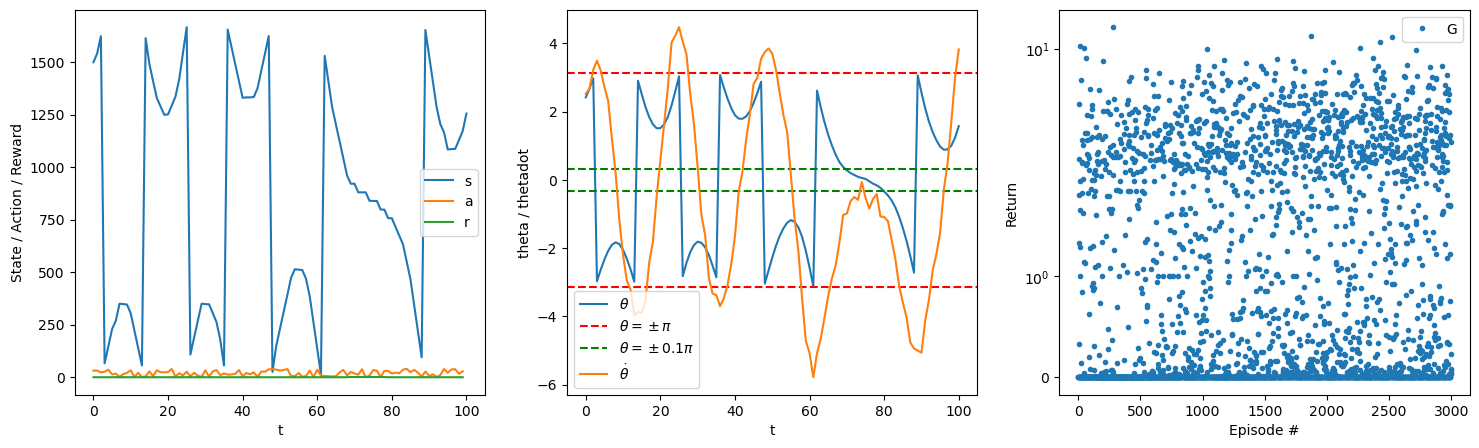
\includegraphics[width=\linewidth]{pendulum/traj_return_sarsa.png}
\caption{Pendulum Trajectory and Learning Curve for SARSA}
\label{fig:pendulum_traj_return_sarsa}
\end{figure}

\begin{figure}[ht]
\centering
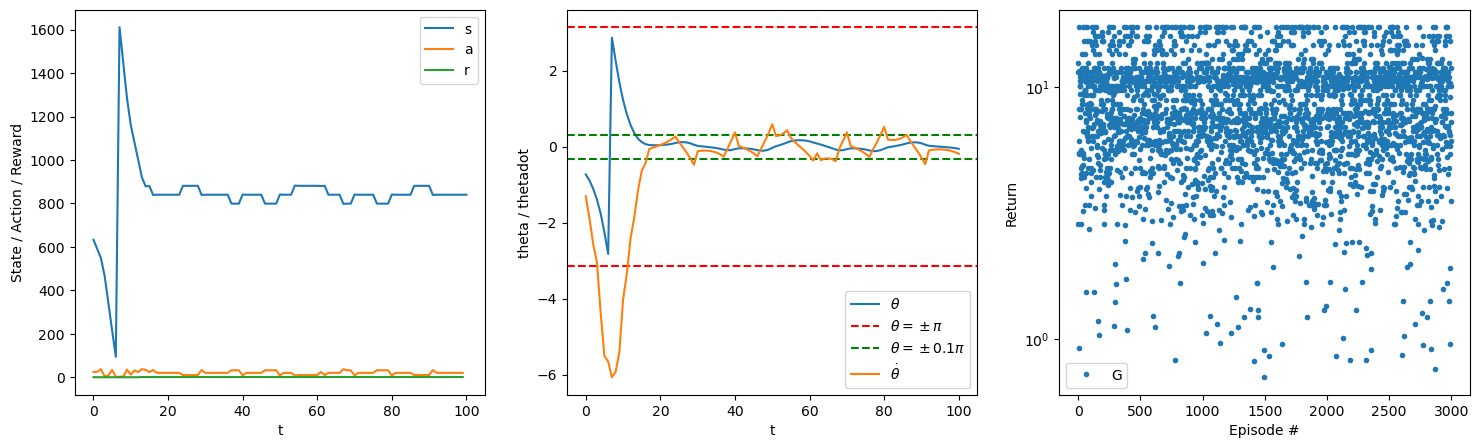
\includegraphics[width=\linewidth]{pendulum/traj_return_td0_sarsa.png}
\caption{Pendulum Trajectory and Learning Curve for SARSA after TD(0)}
\label{fig:pendulum_traj_return_td0_sarsa}
\end{figure}

\begin{figure}[ht]
\centering
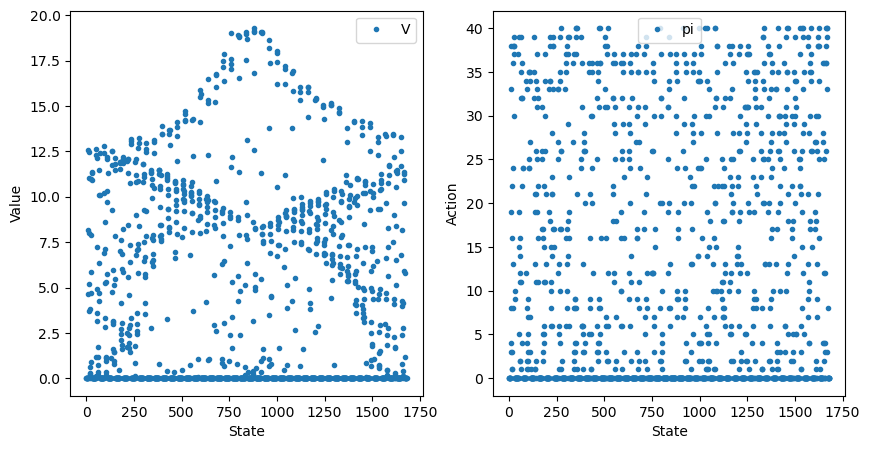
\includegraphics[width=0.8\linewidth]{pendulum/V_pi_sarsa.png}
\caption{Pendulum State Value Function and Policy for SARSA using TD(0)}
\label{fig:pendulum_V_pi_sarsa}
\end{figure}

\begin{figure}
\centering
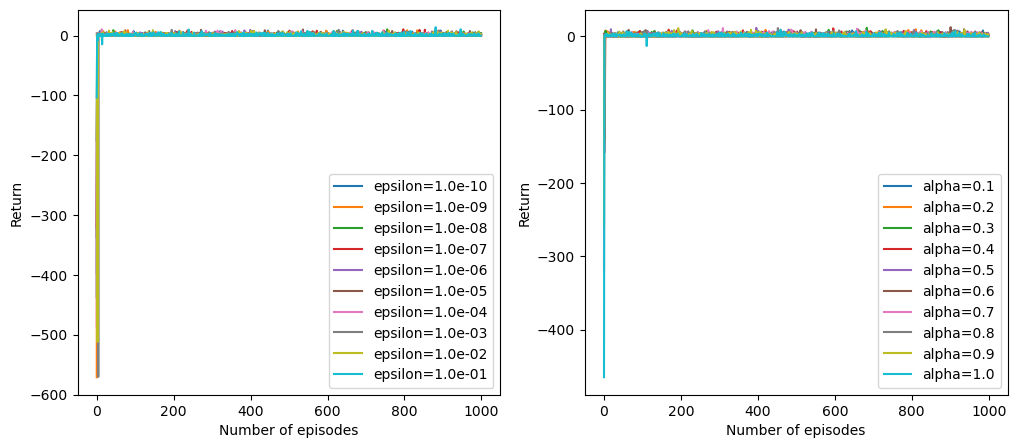
\includegraphics[width=0.8\linewidth]{pendulum/diff_epsilon_alpha_sarsa.png}
\caption{Pendulum Effect of $\epsilon$ and $\alpha$ on Learning Curve for SARSA}
\label{fig:pendulum_diff_epsilon_alpha_sarsa}
\end{figure}

For the pendulum SARSA algorithm, an example trajectory and learning curve are shown in Figure \ref{fig:pendulum_traj_return_sarsa}. The state value function and policy are shown in Figure \ref{fig:pendulum_V_pi_sarsa}. The SARSA algorithm shown here was run for 3000 episodes. Additionally, TD(0) was applied to the SARSA algorithm to derive a state value function. An example trajectory and learning curve are shown in Figure \ref{fig:pendulum_traj_return_td0_sarsa}. For convenience's sake and to understand the learning at different points of the process, Figure \ref{fig:pendulum_traj_return_sarsa} only shows the trajectory at the last iteration of SARSA. Therefore, this case does not perform well. However, the real fruits of the SARSA algorithm can be seen in Figure \ref{fig:pendulum_traj_return_td0_sarsa}, which is a trajectory that uses the policy derived from SARSA. We see here that the pendulum is controlled in 15 time units and remains controlled for the rest of the trajectory. Finally, the effect of varying $\epsilon$ and $\alpha$ on the learning curve is shown in Figure \ref{fig:pendulum_diff_epsilon_alpha_sarsa}. We see that the learning curve is very sensitive to $\epsilon$ and $\alpha$, especially needing high exploration values for $\epsilon$ to gain useful returns.

\subsection*{Q-Learning}
\begin{figure}[ht]
\centering
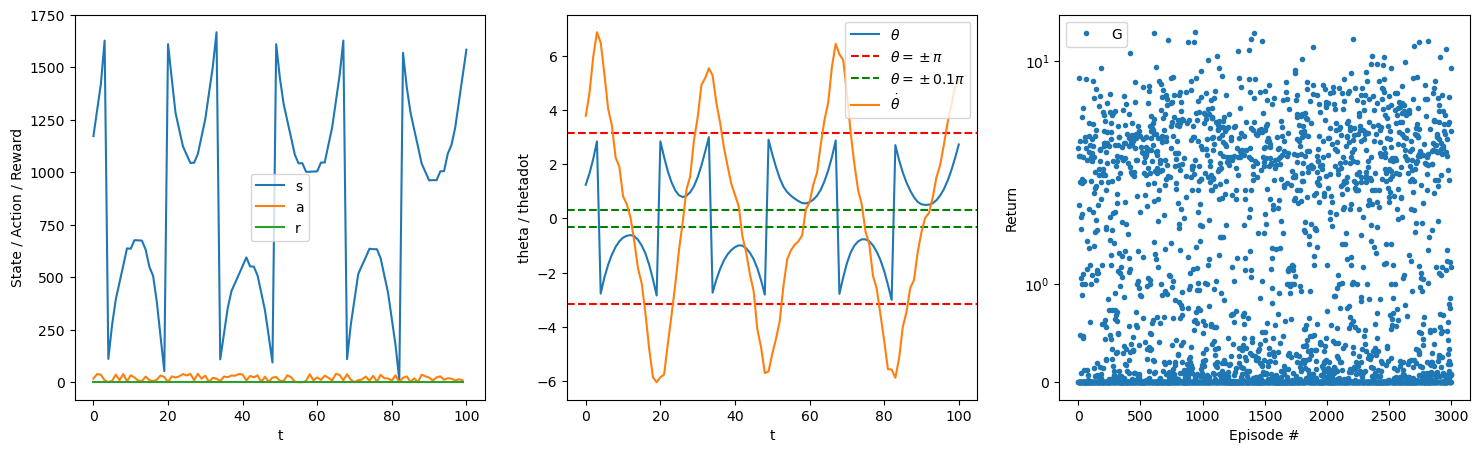
\includegraphics[width=\linewidth]{pendulum/traj_return_q_learning.png}
\caption{Pendulum Trajectory and Learning Curve for Q-Learning}
\label{fig:pendulum_traj_return_q_learning}
\end{figure}

\begin{figure}[ht]
\centering
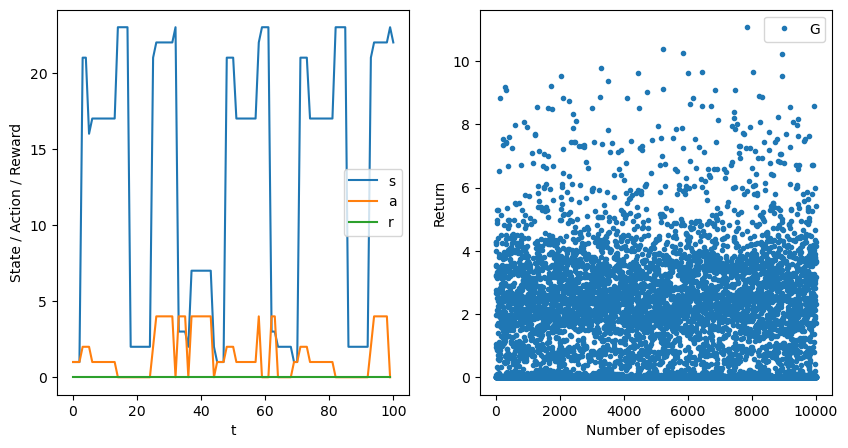
\includegraphics[width=\linewidth]{pendulum/traj_return_td0_q_learning.png}
\caption{Pendulum Trajectory and Learning Curve for Q-Learning after TD(0)}
\label{fig:pendulum_traj_return_td0_q_learning}
\end{figure}

\begin{figure}[ht]
\centering
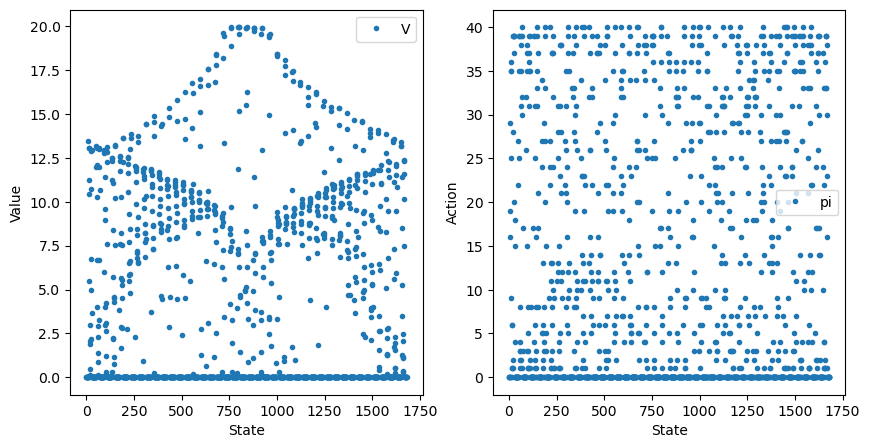
\includegraphics[width=0.8\linewidth]{pendulum/V_pi_q_learning.png}
\caption{Pendulum State Value Function and Policy for Q-Learning using TD(0)}
\label{fig:pendulum_V_pi_q_learning}
\end{figure}

\begin{figure}
\centering
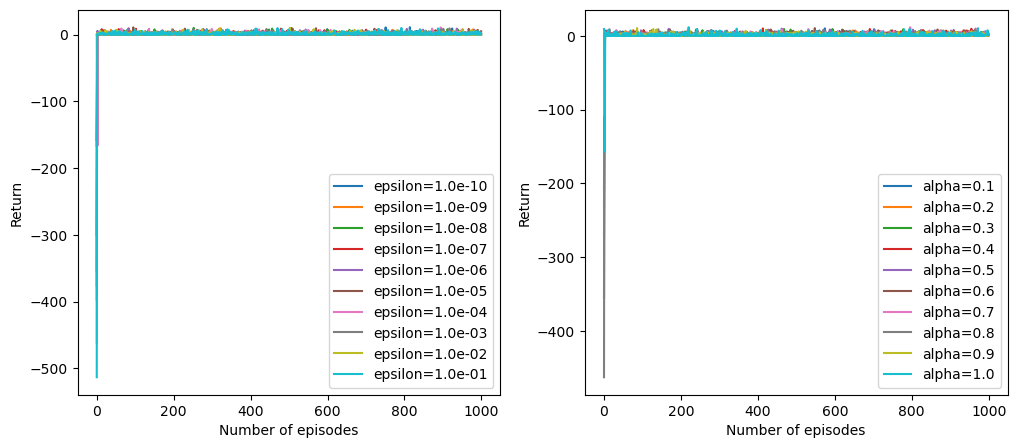
\includegraphics[width=0.8\linewidth]{pendulum/diff_epsilon_alpha_q_learning.png}
\caption{Pendulum Effect of $\epsilon$ and $\alpha$ on Learning Curve for Q-Learning}
\label{fig:pendulum_diff_epsilon_alpha_q_learning}
\end{figure}

For the pendulum Q-Learning algorithm, an example trajectory and learning curve are shown in Figure \ref{fig:pendulum_traj_return_q_learning}. The state value function and policy are shown in Figure \ref{fig:pendulum_V_pi_q_learning}. The Q-Learning algorithm shown here was run for 3000 episodes. Additionally, TD(0) was applied to the Q-Learning algorithm to derive a state value function. An example trajectory and learning curve are shown in Figure \ref{fig:pendulum_traj_return_td0_q_learning}. For convenience's sake and to understand the learning at different points of the process, Figure \ref{fig:pendulum_traj_return_q_learning} only shows the trajectory at the last iteration of Q-Learning. Therefore, this case does not perform well. However, the real fruits of the Q-Learning algorithm can be seen in Figure \ref{fig:pendulum_traj_return_td0_q_learning}, which is a trajectory that uses the policy derived from Q-Learning. We see here that the pendulum is controlled in 15 time units and remains controlled for the rest of the trajectory. Finally, the effect of varying $\epsilon$ and $\alpha$ on the learning curve is shown in Figure \ref{fig:pendulum_diff_epsilon_alpha_q_learning}. We see that the learning curve is very sensitive to $\epsilon$ and $\alpha$, especially needing high exploration values for $\epsilon$ to gain useful returns.


\end{document}
